\documentclass{sigchi}

% Use this command to override the default ACM copyright statement (e.g. for preprints). 
% Consult the conference website for the camera-ready copyright statement.


%% EXAMPLE BEGIN -- HOW TO OVERRIDE THE DEFAULT COPYRIGHT STRIP -- (July 22, 2013 - Paul Baumann)
% \toappear{Permission to make digital or hard copies of all or part of this work for personal or classroom use is 	granted without fee provided that copies are not made or distributed for profit or commercial advantage and that copies bear this notice and the full citation on the first page. Copyrights for components of this work owned by others than ACM must be honored. Abstracting with credit is permitted. To copy otherwise, or republish, to post on servers or to redistribute to lists, requires prior specific permission and/or a fee. Request permissions from permissions@acm.org. \\
% {\emph{CHI'14}}, April 26--May 1, 2014, Toronto, Canada. \\
% Copyright \copyright~2014 ACM ISBN/14/04...\$15.00. \\
% DOI string from ACM form confirmation}
%% EXAMPLE END -- HOW TO OVERRIDE THE DEFAULT COPYRIGHT STRIP -- (July 22, 2013 - Paul Baumann)


% Arabic page numbers for submission. 
% Remove this line to eliminate page numbers for the camera ready copy
\pagenumbering{arabic}


% Load basic packages
\usepackage{balance}  % to better equalize the last page
\usepackage{graphics} % for EPS, load graphicx instead
\usepackage{times}    % comment if you want LaTeX's default font
\usepackage{url}      % llt: nicely formatted URLs

% llt: Define a global style for URLs, rather that the default one
\makeatletter
\def\url@leostyle{%
  \@ifundefined{selectfont}{\def\UrlFont{\sf}}{\def\UrlFont{\small\bf\ttfamily}}}
\makeatother
\urlstyle{leo}


% To make various LaTeX processors do the right thing with page size.
\def\pprw{8.5in}
\def\pprh{11in}
\special{papersize=\pprw,\pprh}
\setlength{\paperwidth}{\pprw}
\setlength{\paperheight}{\pprh}
\setlength{\pdfpagewidth}{\pprw}
\setlength{\pdfpageheight}{\pprh}

% Make sure hyperref comes last of your loaded packages, 
% to give it a fighting chance of not being over-written, 
% since its job is to redefine many LaTeX commands.
\usepackage[pdftex]{hyperref}
\hypersetup{
pdftitle={SIGCHI Conference Proceedings Format},
pdfauthor={LaTeX},
pdfkeywords={SIGCHI, proceedings, archival format},
bookmarksnumbered,
pdfstartview={FitH},
colorlinks,
citecolor=black,
filecolor=black,
linkcolor=black,
urlcolor=black,
breaklinks=true,
}

% create a shortcut to typeset table headings
\newcommand\tabhead[1]{\small\textbf{#1}}


% End of preamble. Here it comes the document.
\begin{document}

\title{Striving for Perfection: Measurement of Incremental Fitness Improvement}

\numberofauthors{2}
\author{
  \alignauthor Meg Quintero\\
    \affaddr{Harvard University}\\
    \affaddr{514 Kirkland Mail Center, Cambridge, MA}\\
    \email{mmquint@college.harvard.edu}
  \alignauthor Vladimir Bok\\
    \affaddr{Harvard University}\\
    \affaddr{117 Eliot Mail Center, Cambridge, MA}\\
    \email{vladimirbok@college.harvard.edu}
}

\maketitle

\begin{abstract}
TBA
\end{abstract}

\keywords{
	Kinect; Metabolic Conditioning;
}

\section{Introduction}

\subsection{Motivation}
Intensive workout programs such as P90x, Insanity, and Rushfit promise users to transform their bodies into the “best shape of their life” by following a 60 to 90 days workout regimen.  These types of routines feature methodologies such as “Muscle Confusion,” “Max Interval Training,” or “High Intensity Interval Training,” which all fall into the Metabolic Conditioning exercise category---exercises that increase the storage and delivery of energy for any activity through the improvement of strength and endurance.  While a multitude of users report great results, many do not endure long enough to reap the fitness benefits of these programs. Prior research (see related work section) has shown that motivation improves exercise adherence. Accordingly, it is our belief that one of the main reasons people fail to persevere these exercise regimen is the lack of observable progress from one workout to the next, a crucial motivating factor. Unlike strength training exercises--such as bench press or deadlift--the incremental improvements of Metabolic Conditioning workouts are often not apparent until weeks into the program, causing many users to lose motivation and quit the program early in the 60-90 days regimen. The goal of our study is to leverage motion tracking devices such as the Microsoft Kinect to create a software tool for calculating incremental progress for Metabolic Conditioning exercises and ultimately motivate users to adhere to their Metabolic Conditioning routine of choice.

\subsection{Approach}
The intensity of a MC type exercise movement can be measured by the amount of resistance (either body resistance or use of external weights), the volume of repetitions performed and the power or rate at which work is performed. It is our goal to use relatively inexpensive technology, such as the Microsoft Kinect, to measure exerciser’s progress with a reasonable accuracy.
We have met with our fitness experts to create a workout in the style of P90x and Insanity that features exercises that fit the following criteria:
\begin{itemize}
	\item Requires little to no prior skill or training 
	\item Requires strength to accurately achieve the best stance for that particular move
	\item Requires stamina to complete the exercise move at a fast rate.
\end{itemize}
The primary goal of our first set of user studies was to perfect our post processing models and isolate and fix any flaws with the study itself, however, a secondary goal was to collect real data that could inspire our fitness expert benchmark data.  To establish this expert benchmark data set, we used an accumulation of the first set of participants' performance and the knowledge gained from meeting with the experts.  \\
We recorded both the video footage of each participant completing the routine as well as the skeleton and depth sensor data collection tool created to measure factors such as rate of exercise move, body form (predominantly angles between limbs and differences in vertical and horizontal movement), speed, height (where applicable), the duration and frequency of resting time, and the volume of repetitions performed.  We then calculated a score or percentage of the expert benchmark using the collected data as well as generating more granular data specific to each workout move completed.  After the participant has finished the workout, we showed them two different reports 1.) The expert percentage score and 2.) The granular exercise move specific report and ask them to determine which report would be most helpful for them in terms of tracking their performance from workout to workout.

\subsection{Contribution}
If successful, our work will show that currently hard to benchmark exercises can be evaluated in terms of performance with relatively inexpensive hardware.  We predict that our measurement tool could be meaningful to potential users to track minute performance improvements and, ultimately, inspire them to continue working towards their fitness goals.  Much research has already been done regarding measuring exercise performance using technology that has inspired and motivated this research project.  We believe our work addresses a hole in this field that has not been explored that we believe will spark future work in the field of exercise motivation and progress analysis through the use of inexpensive technology.

\section{Related Work}
The notion of tracking one's progress and quantifying improvement is an old one. As early as the 18th century, Benjamin Franklin kept a daily journal to monitor his performance in thirteen personal virtues. 
% CITATION
%%%
Modern research provides formal basis for what Benjamin Franklin seemed to know intuitively: the idea that measurement improves adherence and ultimately promotes long-term behavioral change. For example, Dr. Melody Noland measured the effects of self-monitoring and reinforcement on adherence to unsupervised exercise
\cite{Noland1989Effects}. 
Splitting the study subjects into three groups (self-monitoring, reinforcement supplied by another person, and control), she found that the self-monitoring and reinforcement groups reported a significantly higher frequency of exercise and better results than the control group 
\cite{Noland1989Effects}. % CITATION
%%%
Despite the encouraging results, Dr. Noland's methodology may today seem outdated: the self-monitoring subjects were required to keep a written log of their exercise
\cite{Noland1989Effects}, % CITATION
leaving much to be desired in terms of usability and automation of what may otherwise be a very tedious process. Indeed, the decade following the 1989 publication of Dr. Nolan’s research witnessed the onset of persuasive technologies, which likewise leveraged progress tracking as a means of sustaining desired behavior. 
%%%
One of the pioneers of the field, Dr. Sunny Consolvo and her co-authors explored the ways in which technology could be used to encourage behavioral change
\cite{Consolvo2009Theory, Consolvo2008Flowers}. % CITATION
In ``Theory-Driven Design Strategies for Technologies that Support Behavior Change in Everyday Life", Consolvo et. al. did an excellent job drawing on prior research in behavioral psychology and situating their work in the context of relevant psychology theories. For instance, the Goal-Setting Theory stresses the importance of an ongoing feedback as progress is made as opposed to merely providing a reward when a goal is achieved 
\cite{Consolvo2009Theory}. % CITATION
Choosing data abstraction as one of the main design tenets of UbiFit, the software they created for the purposes of their study, Consolvo et. al. implemented an animated garden that tracks and encourages progress toward the desired goal 
\cite{Consolvo2009Theory, Consolvo2008Flowers}. % CITATION
%%%
Our research takes a different approach by instead enabling the measurement of granular, incremental changes that the UbiFit garden interface does not capture. As such, our research enters a contented field of performance measurement tracking devices. Indeed, those interested in physical activity tracking devices have a myriad of options, such as Jawbone Up, Fitbit, or the Nike Fuel Band, all of which offer different ways of performance tracking. Relying predominantly on accelerometers, theses devices fail to account for improvements in form and are prone to count mindless handshaking toward the user's exercise score with much opportunity for the user to game the system. Unlike these commercial devices, our goal is to use Microsoft Kinect to develop exercise-tracking software that could accurately measure the incremental qualitative improvements in a person's form and overall execution of an exercise routine, rather than a raw quantity of physical activity in insolation.



\section{Methodology}
TBA

\subsection{Workout Routine}
The participants each performed three sets of exercises moves.  Each set contained three different moves and each was done for a total of 30 seconds.  After a participant completed the three moves, they performed the "resting move" for a total of 60 seconds and then repeated the set.  The three sets are as follows:
\begin{enumerate}
	\item Set 1
	\begin{enumerate}
		\item Move 1: Jumping Jacks
		\item Move 2: Arm Circles
		\item Move 3: Knee to Elbows
	\end{enumerate}
	\item Set 2
		\begin{enumerate}
		\item Move 1: Squat Jumps
		\item Move 2: Side to Side Jumps
		\item Move 3: High Marches
	\end{enumerate}	
	\item Set 3
	\begin{enumerate}
		\item Move 1: Jumping Jacks
		\item Move 2: Arm Circles
		\item Move 3: Tuck Jumps
	\end{enumerate}
\end{enumerate}

\subsection{Micosoft Kinect Data Collection}
TBA

\subsection{Post Processing}

After movement data were collected, we ran our analysis to compute volume rates for each exercise and form measurement for three selected exercises: jumping jacks, high marches, and squat jumps. Below we describe the data analysis procedures we performed. (The first step, omitted from the descriptions below, was essential data cleansing by deleting rows containing NULL values. The number of such rows did not exceed two per any of the data files, amounting to less than 0.002\% of the data.)

\subsubsection{Rate Calculations}
\textbf{Jumping Jacks}  \\
Jumping jacks consist of starting position (standing still, feet together) and jumping position (feet spread wide). To compute repetitions, we took the x coordinates of a participant's left and right feet and plotted the absolute difference between the two coordinates over time, as shown in figure below.
%%%%%%%%%%%%%%%%%%%%%%%%%%
\begin{figure} [htp]
	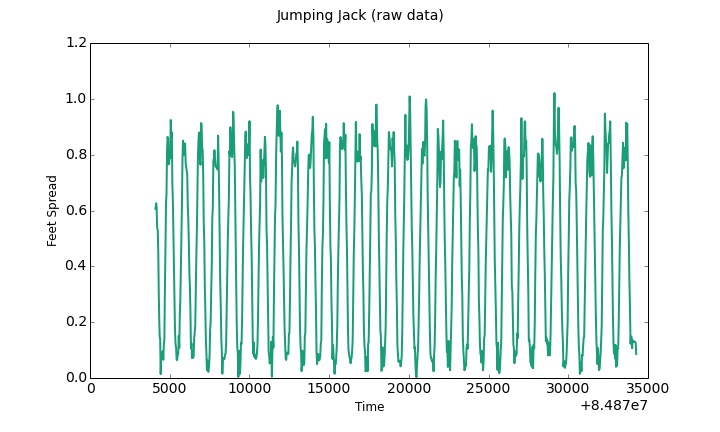
\includegraphics[width=0.5\textwidth]{images/jj_raw}
%\caption{Arm Circles Results}
\end{figure}
%%%%%%%%%%%%%%%%%%%%%%%%%%
Each of the lows corresponds to a starting position and each of the peaks corresponds to a jumping position. Therefore, to count the number of repetitions, it suffices to count the number of peaks. Given the relative noisiness of the original data set, a naive algorithm to compute local maxima would yield an excessive number of false positives, necessitating further data processing. We experimented with two methods: smoothing and robust peak detection. In terms of smoothing, we applied a third-order spline interpolation. For robust peak detection, we classified a point as a local maximum if and only if it was preceded by a value lower than some delta, using an algorithm provided by Eli Billauer \cite{Billauer}. The best value of delta was determined by trial-and-error using our training data set consisting of three subjects (this data set was kept separate from our study data set). While each of theses methods led to significant improvements by itself, as determined by a dramatic reduction in the number of false positives, we found that we obtained the best results when we used both techniques: First, we smoothed-out the data, and then we applied the peak detection algorithm. Figure below shows the curve after smoothing. To compute the rate, we took the number of detected peaks and divided by the duration of the exercise.
%%%%%%%%%%%%%%%%%%%%%%%%%%
\begin{figure} [htp]
	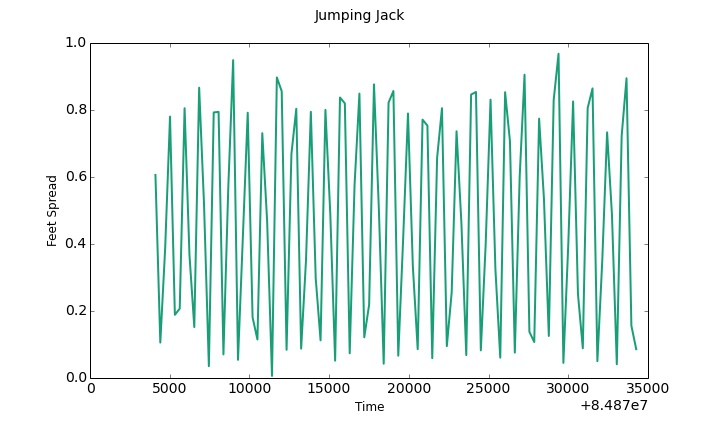
\includegraphics[width=0.5\textwidth]{images/jj}
%\caption{Arm Circles Results}
\end{figure}
%%%%%%%%%%%%%%%%%%%%%%%%%%

\textbf{Squat Jumps}  \\
Similarly to jumping jacks, squat jumps consist of two basic positions: regular squat (starting posture) and a jump. To measure repetitions, we took the average y-coordinate values of a participant's feet and plotted the averages over time. As anticipated, the data revealed a pattern with distinct peaks, corresponding to each of the jumps. Figure below shows the curve after smoothing.
%%%%%%%%%%%%%%%%%%%%%%%%%%
\begin{figure} [htp]
	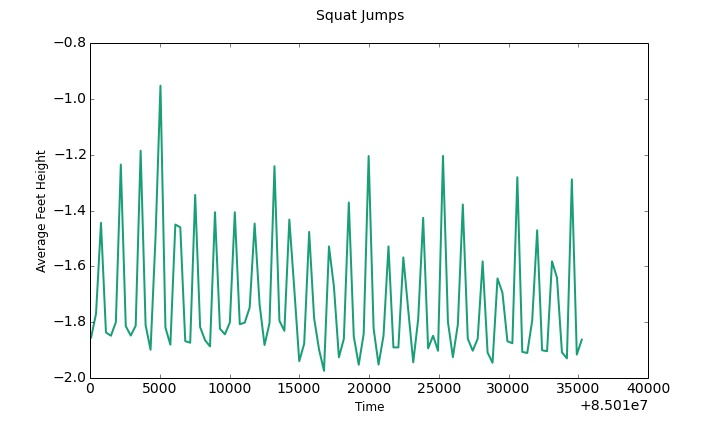
\includegraphics[width=0.5\textwidth]{images/sj}
%\caption{Arm Circles Results}
\end{figure}
%%%%%%%%%%%%%%%%%%%%%%%%%%
As in processing jumping jacks, we applied the peak detection algorithm on the smoothed-out curve, obtaining the number of repetitions, and then divided the count by exercise duration, to obtain the rate.

\textbf{High Marches} \\
High marches consist of alternatively kicking up as high as possible right and left feet, preferably while keeping knees straight. In analyzing high marches, we considered each leg separately. We took the y-coordinates of left and right ankles, smoothed-out the data and plotted it over time time. Figures below shows the curve for right ankle after smoothing. As in our earlier analyses, the number of peaks gave the number of repetitions, which we divided by duration to obtain the rate.
%%%%%%%%%%%%%%%%%%%%%%%%%%
\begin{figure} [htp]
	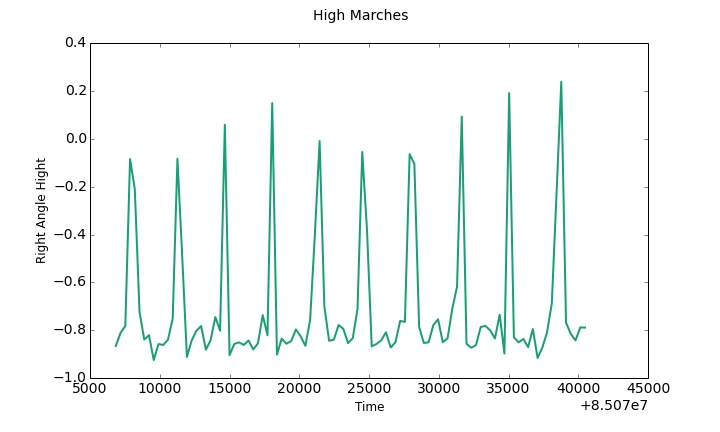
\includegraphics[width=0.5\textwidth]{images/hm}
%\caption{Arm Circles Results}
\end{figure}
%%%%%%%%%%%%%%%%%%%%%%%%%%

\textbf{Side-to-Side Jumps} \\
As the name suggests, side-to-side jumps consist of jumping from left to right, while keeping feet together. To calculate the rate, we took the average x-position of a participant's feet, smoothed-out the data, and plotted it over time. Then, we computed the number of peaks (corresponding to the time when the participant's feet were at rightmost point) and lows (corresponding to the time when the participant's feet were at the leftmost point). Figures below shows the curve after smoothing. We then used the sum of those numbers divided by exercise duration to obtain the rate.
%%%%%%%%%%%%%%%%%%%%%%%%%%
\begin{figure} [htp]
	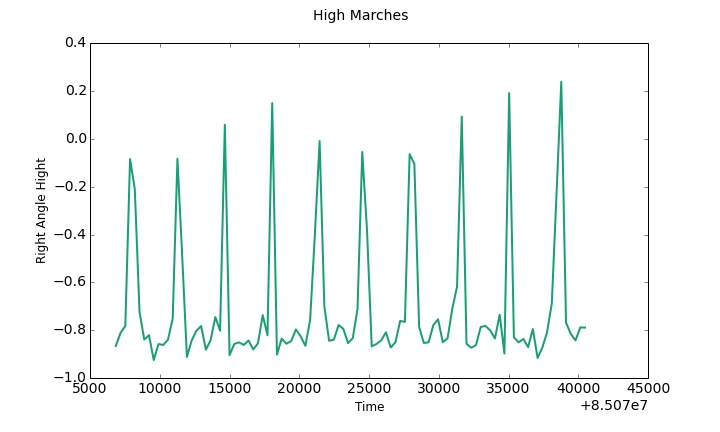
\includegraphics[width=0.5\textwidth]{images/hm}
%\caption{Arm Circles Results}
\end{figure}
%%%%%%%%%%%%%%%%%%%%%%%%%%

\textbf{Knee to Elbow} \\
To perform knee-to-elbow, a participant twists his torso while lifting his left knee to touch his right elbow, and then repeats on the opposite side, bringing up his right knee to touch his left elbow. From the standpoint of rate calculation, this exercise was more challenging to compute than any of the prior four. We took the x and y coordinates of a participant's left knee and right elbow. Then, we computed the Euclidean distance of these points over time. We repeated the same for right knee and left elbow and plotted the differences over time. Figures below shows the curve after smoothing. The lows correspond to the points when the participant's knee was closest to the corresponding elbow---indicating a completed repetition. Accordingly, we counted the number of lows on the smoothed-out curves for both knee-elbow pairs using the same strategy we used to detect peaks. A sum of those lows was then used to compute the rate.
%%%%%%%%%%%%%%%%%%%%%%%%%%
\begin{figure} [htp]
	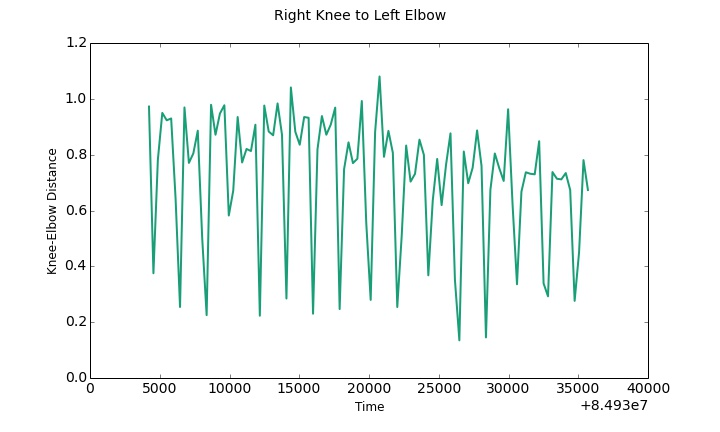
\includegraphics[width=0.5\textwidth]{images/ke}
%\caption{Arm Circles Results}
\end{figure}
%%%%%%%%%%%%%%%%%%%%%%%%%%

\textbf{Tuck Jumps} \\
Tuck jumps require the participant to jump as high as he or she can, raising his or her knees up. Here, we plotted the average y-position of the participant's knees over time; accordingly, each peak corresponds to a completed jump. Figures below shows the curve after smoothing. Similarly to the above-described procedures, we used the number of peaks to compute the rate.
%%%%%%%%%%%%%%%%%%%%%%%%%%
\begin{figure} [htp]
	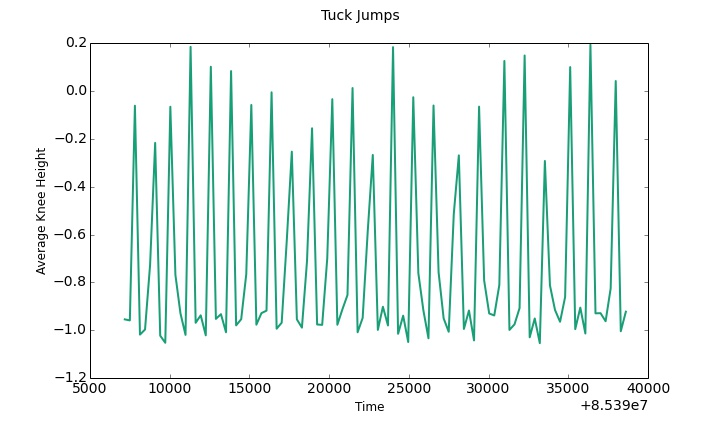
\includegraphics[width=0.5\textwidth]{images/tj}
%\caption{Arm Circles Results}
\end{figure}
%%%%%%%%%%%%%%%%%%%%%%%%%%

\textbf{Arm Circles} \\
In arm-circles starting position, the participant stands upright with arms extended to his or her sides, parallel to the ground. To perform the exercise, the participant makes circles with his or her outstretched arms, keeping elbows locked. To determine the number of repetitions, we observed that participant’s hand follows a roughly circular trajectory in the yz-plane. During a single circular traversal, a hand reaches exactly one minimum and maximum y and z position. Therefore, we plotted the smoothed-out the z and y positions for each wrist and computed the count of peaks and lows for each, dividing by two to obtain number of repetitions per wrist. Figures shows the curve for right wrist after smoothing. (While it would have been computationally simpler to consider only one of the dimensions---y or z---for the purposes of counting, such estimation could be easily deceived by up-down or front-back movement instead of the proper circular one.) We then took the average of the per-wrist repetition counts to compute the overall rate for this exercise.
%%%%%%%%%%%%%%%%%%%%%%%%%%
\begin{figure} [htp]
	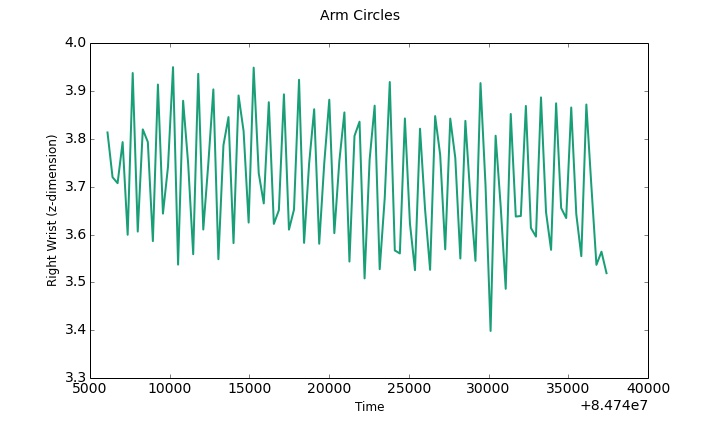
\includegraphics[width=0.5\textwidth]{images/ac}
%\caption{Arm Circles Results}
\end{figure}
%%%%%%%%%%%%%%%%%%%%%%%%%%

\subsubsection{Form Measurement}

In addition to counts, we developed ways to compute form metrics for select three exercises---jumping jacks, high marches, and squat jumps. We describe our methodology below.

\textbf{Jumping Jacks} \\
A proper form for jumping jacks demands straight knees throughout the exercise, wide leg spread in the jumping position, and complete retreat to the starting position where feet are touching. We noticed that all of these characteristics closely correlate with the magnitude of the difference between a participant's right and left feet x positions. For instance, a participant cannot achieve as large a spread in the jumping position if his knees are not straight compared to when his knees are locked. In addition, the differences will be smaller if the participant fails to retreat completely to the starting position before performing another jump. Accordingly, we used the average difference of the x coordinates of a participant's left and right feet, normalized by the his height, to gauge relative form between participants.

\textbf{High Marches} \\
To perform high marches properly, a participant needs to kick up as high as possible while keeping her knees straight. Unfortunately, the knee data have shown to be too noisy to make fine deductions such as the relative straightness of knees. However, we observed that bent knees necessarily lead to lower feet y-position during kick-ups compared to when the knees are straight. Therefore, we used the average foot height per each rep, normalized by the participant's height, to compute the relative form metric for high marches.

\textbf{Squat Jumps} \\
Squat jumps demand that the participant jumps as high as possible while bringing his or her knees as close to his or her chest as possible. Accordingly, to compute a metric that could be used to compare squat jump form across multiple participants, we took the average in-jump knee height for each participant, normalized by height.



\subsection{Feedback}
After completion of the exercise routine, we presented each participant with two types of feedback. First, a holistic one, which consisted of two percentages summarizing how the participant performed relative to our expert benchmark: rate percentage alone and rate percentage after accounting for form.  Second, a granular one comprising a detailed output of our data processing, including graphs and rates for each exercise. We then asked which type of feedback the participant would find most helpful as a means of tracking progress and improvement over time, and recorded their response. 


\subsection{Participants}
TBA

\section{Results}
%%TBA

\subsection{Quantitative Results}
To measure quantitative accuracy of our model, we took a video recording of each of our participants. We then manually counted the number of repetitions for each of the exercises in our routine and compared them to the count estimates given by our model. The figures below show our results as 100\% stacked column charts. If our model performed accurately, both the ''Actual'' and the ''Estimated'' bars would account for 50\% each. If the ''Estimated'' bar comprises less than 50\%, it means our model underestimated the total count; correspondingly, if the ''Estimated'' bar takes up over 50\%, it means our model overestimated. For reference, we also included a table detailing the counts under each of the graphs.\\
\begin{figure} [htp]
	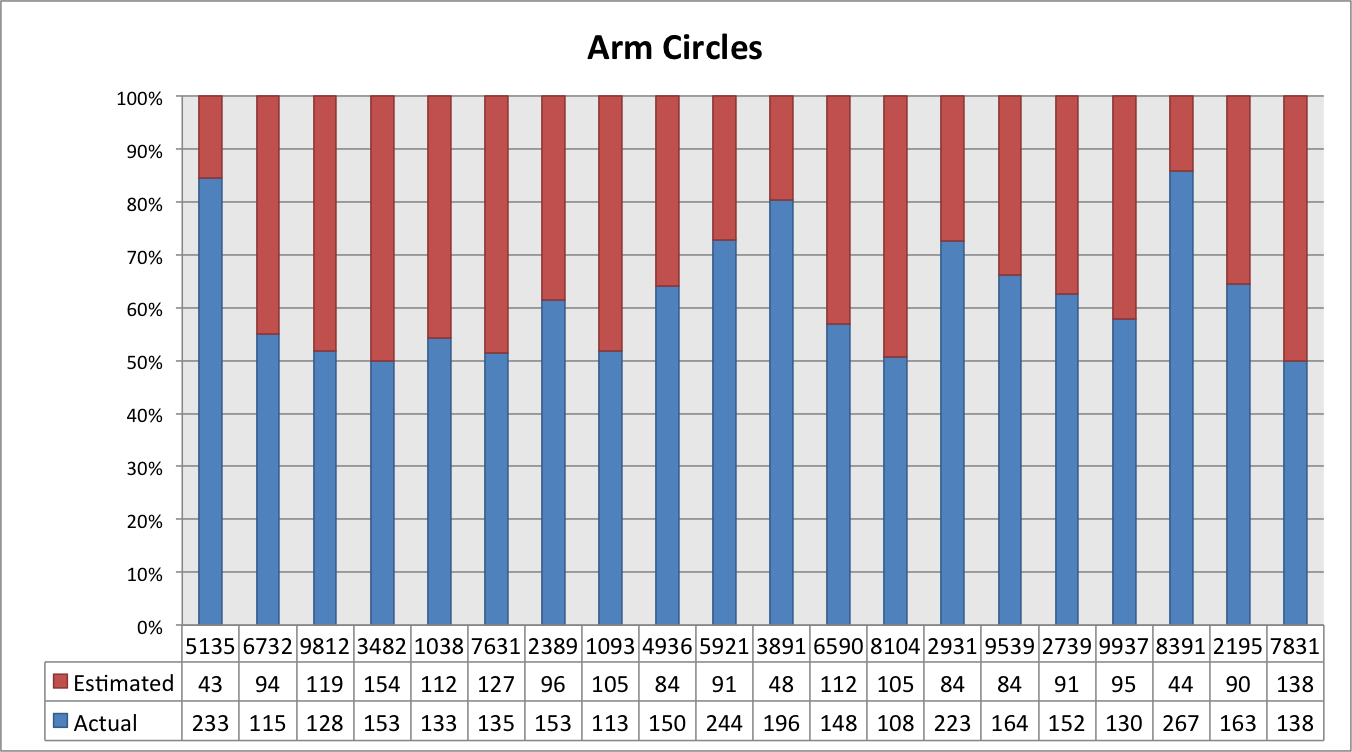
\includegraphics[width=0.5\textwidth]{images/armcircles}
\caption{Arm Circles Results}
\end{figure}
\begin{figure}[htp]
	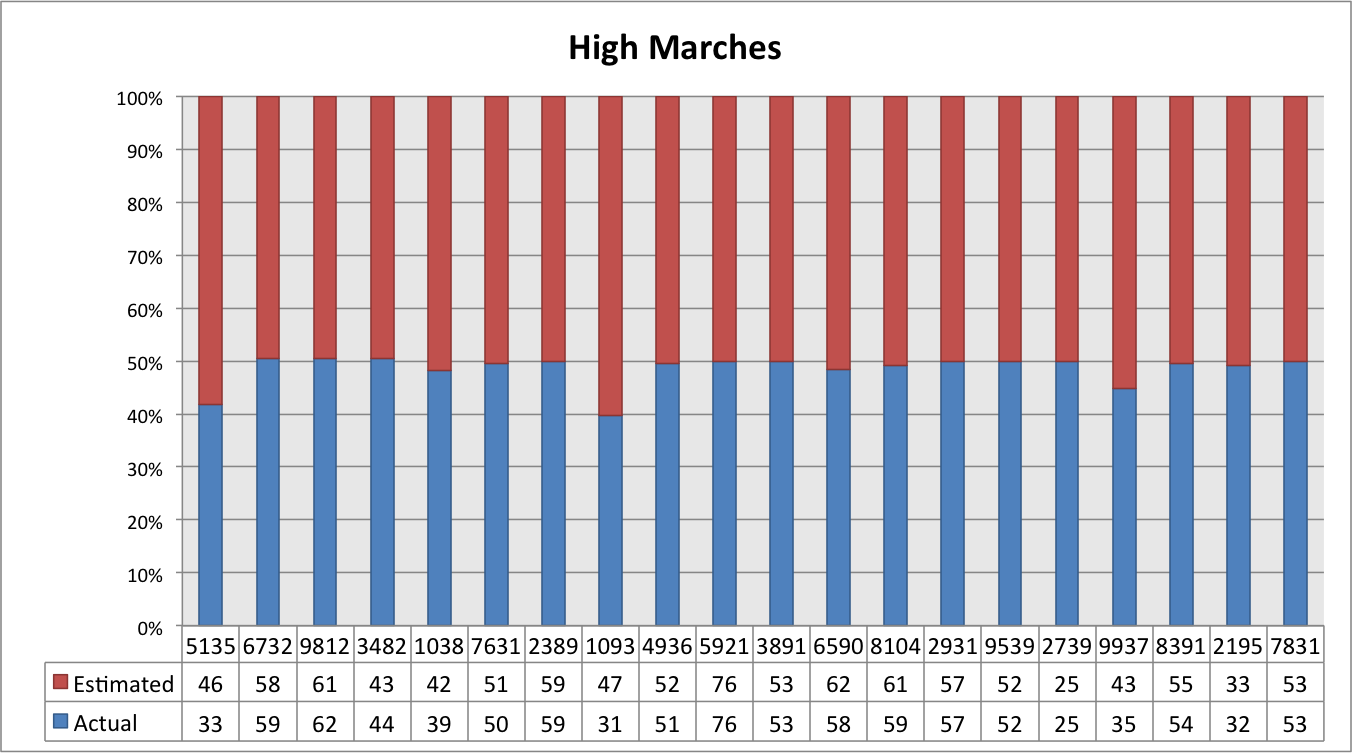
\includegraphics[width=0.5\textwidth]{images/highmarches}
\caption{High Marches Results}
\end{figure}
\begin{figure} [htp]
	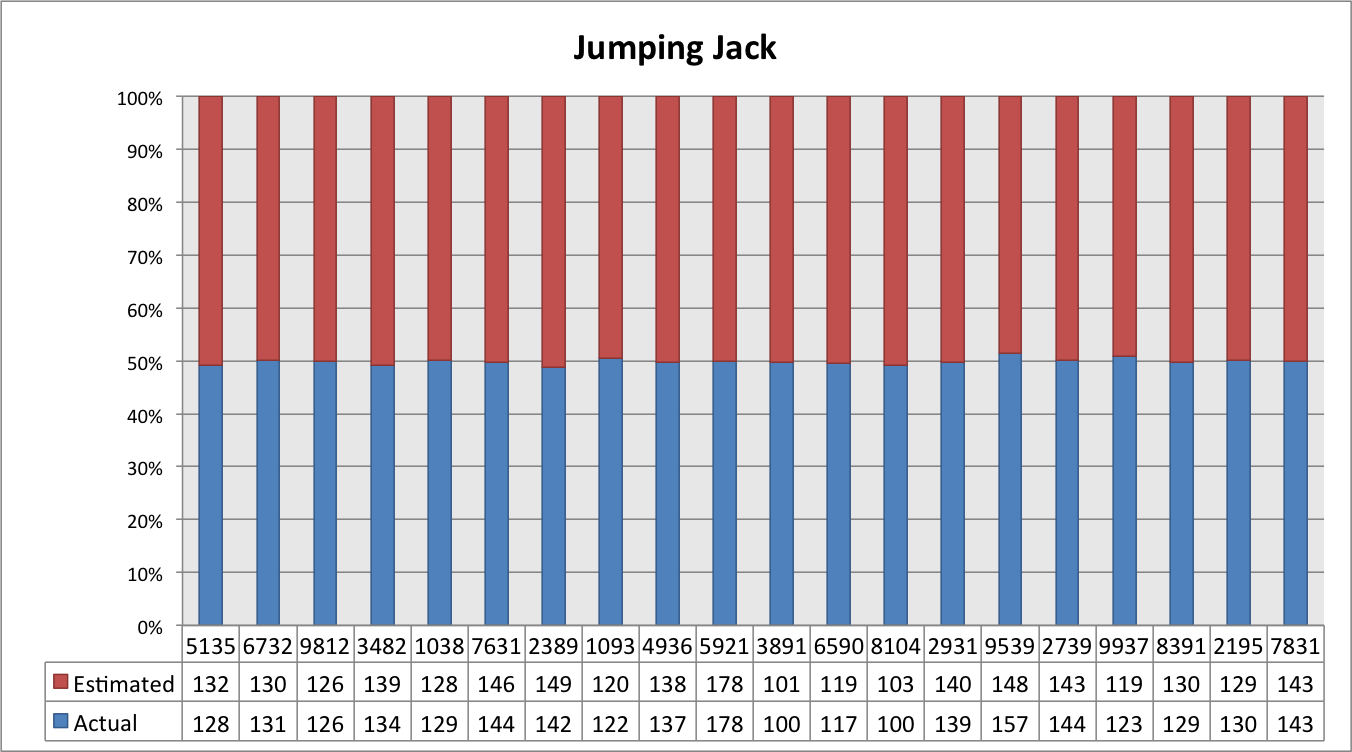
\includegraphics[width=0.5\textwidth]{images/jumpingjack}
\caption{Jumping Jacks Results}
\end{figure}
\begin{figure} [htp]
	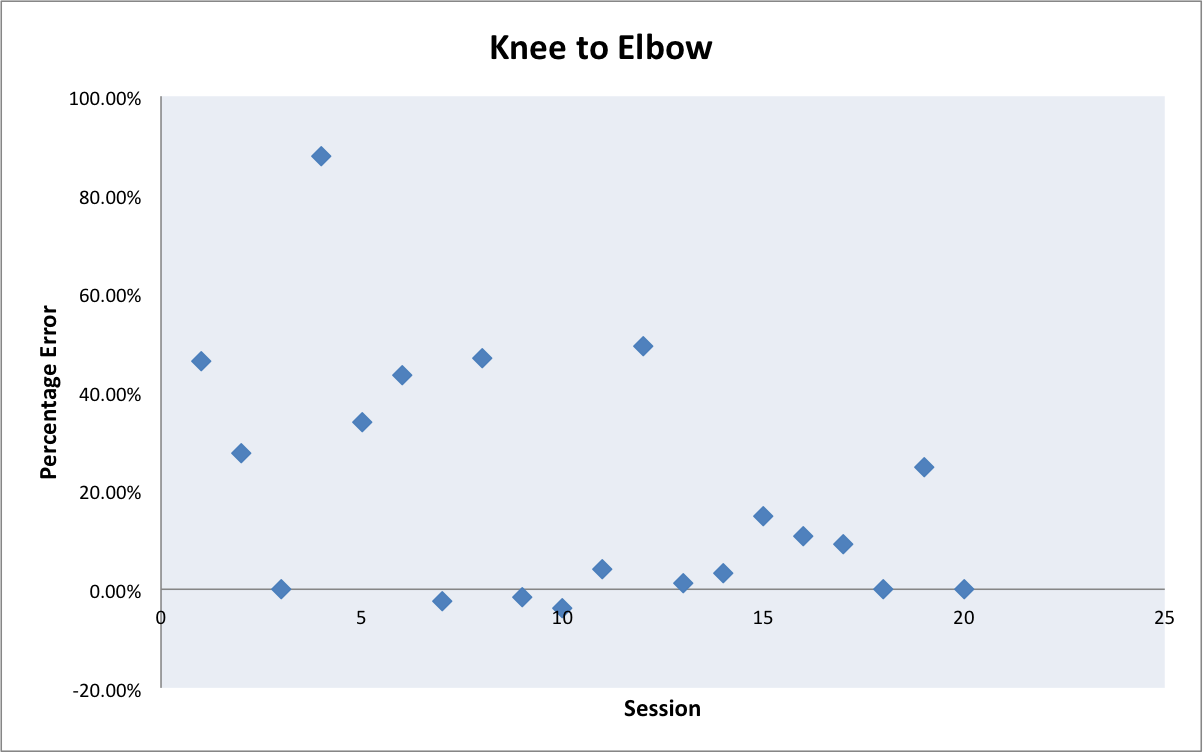
\includegraphics[width=0.5\textwidth]{images/kneetoelbow}
\caption{Knee to Elbow Results}
\end{figure}
\begin{figure} [htp]
	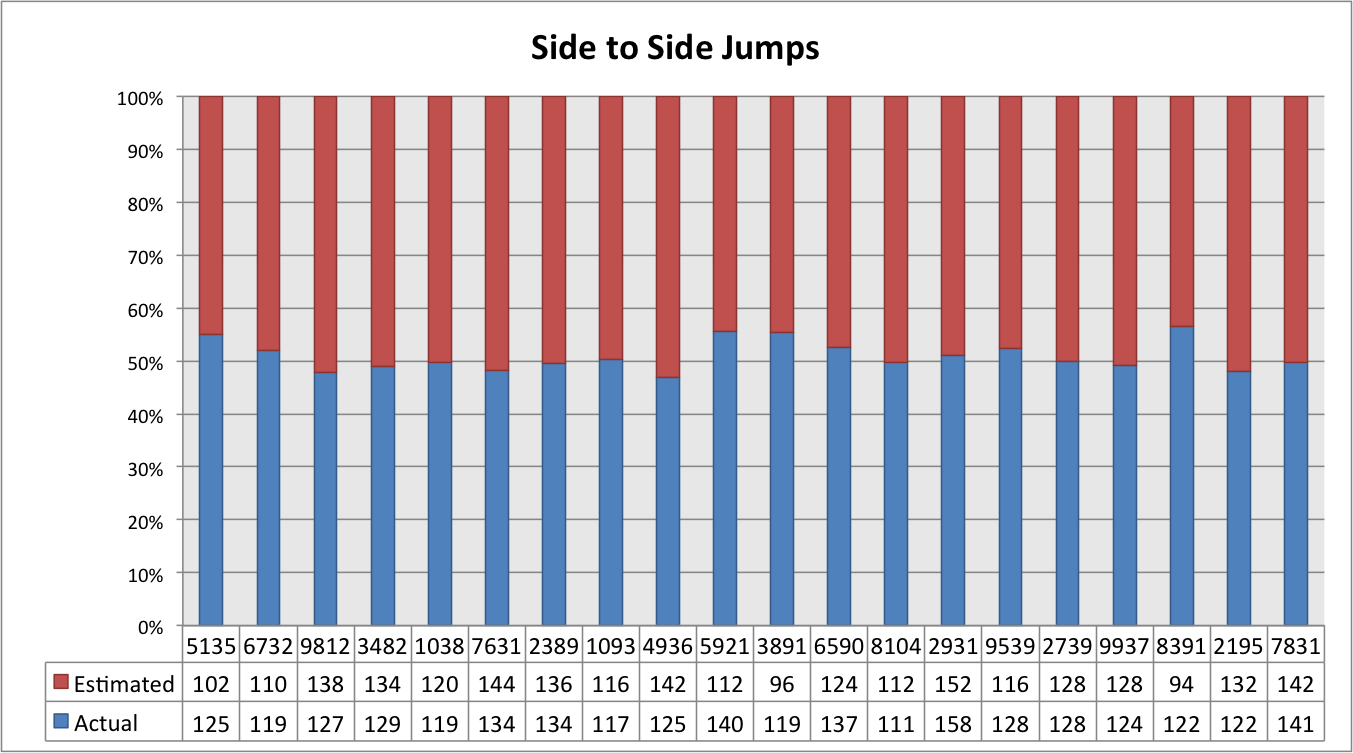
\includegraphics[width=0.5\textwidth]{images/sidetoside}
\caption{Side to Side Results}
\end{figure}
\begin{figure} [htp]
	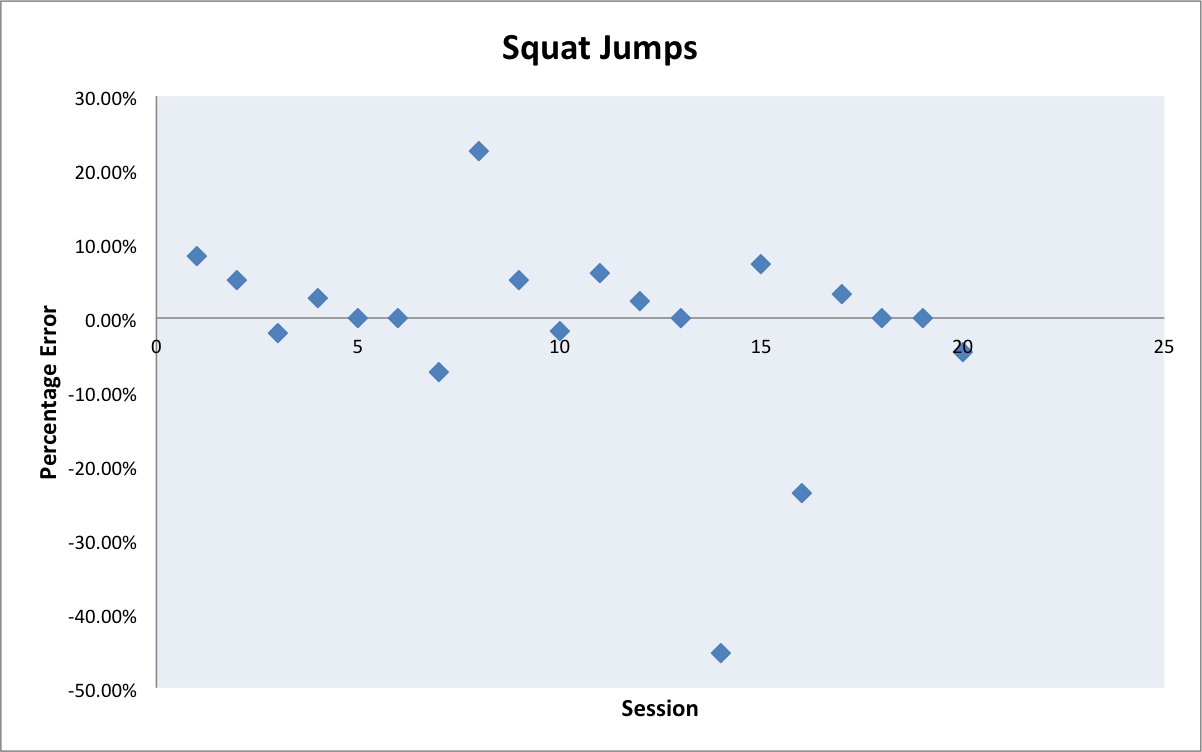
\includegraphics[width=0.5\textwidth]{images/squatjumps}
\caption{Squat Jumps Results}
\end{figure}
\begin{figure} [h!]
	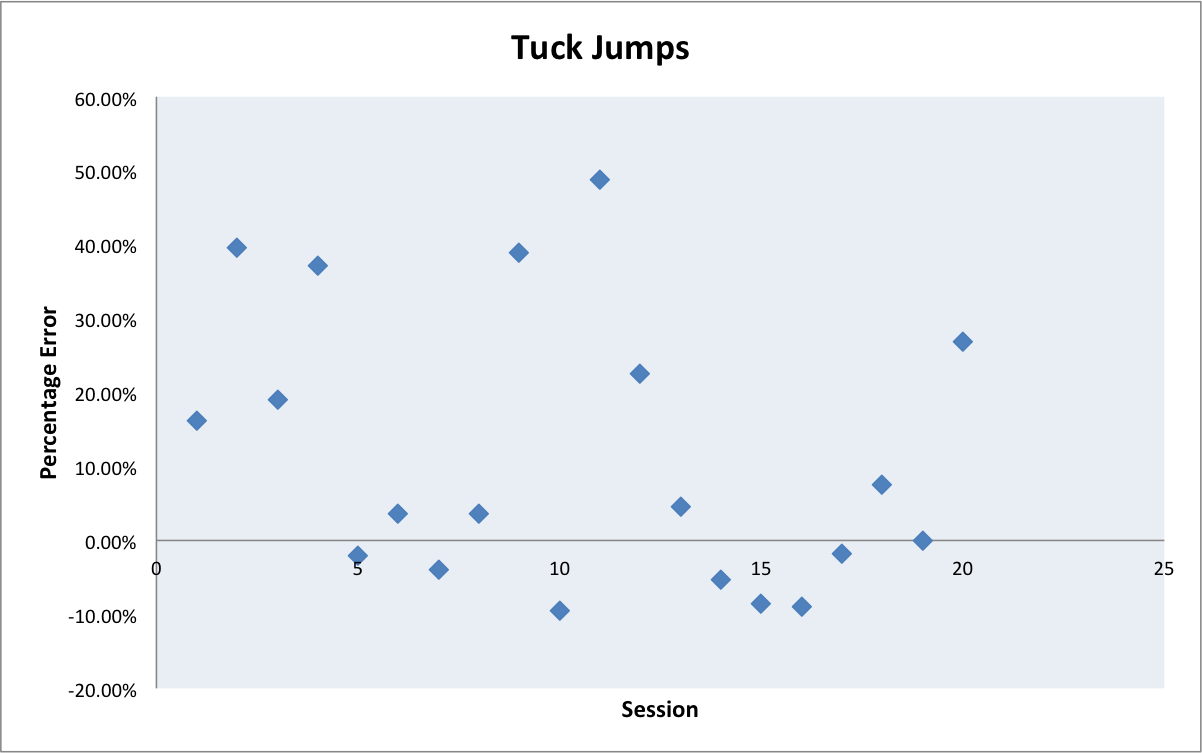
\includegraphics[width=0.5\textwidth]{images/tuckjumps}
\caption{Tuck Jumps Results}
\end{figure} 
Clearly, our model gave more accurate count estimates for certain exercise (such as jumping jacks) and less accurate estimates for others (such as arm circles). Another observation we can make is that the bias in our model is not random but tends to either overestimate most of the time or underestimate most of the time. A discussion of the possible explanations for the performance disparities and inaccuracies is left for the Discussion section. \\

\subsection{Qualitative Results}
In order to measure the qualitative and quantitative accuracy of our performance models, we enlisted the help of 3 experts in the field of fitness that are currently employeed by the Harvard athletic department (see acknowledgments for specific titles).  One of the most important goals of our project was to succeed in terms of relative performance ranking, (i.e. the expert score percentage assigned to each participant based on their performance) was not as important as the ability to successfully compare the form and performance of participants in relation to each other.  For each of the four performances regarding form (Jumping jacks, high marches, squat jumps, and overall performance adjusted by form), the 20 participants were sorted in order of descending performance score.  Groupings were then formed based on rank and the percentage difference in ranking.  The three ranking pairs choosen were the following: \\
\begin{itemize}
	\item{1st and 20th, 95\% difference in ranking} \\
	\item{5th and 16th, 55\% difference in ranking} \\
	\item{9th and 12th, 15\% difference in ranking} 
\end{itemize}
For the three specific exercise moves, the experts were shown 30 seconds of footage for each of the two participants performing the move in the ranking pair.  The experts were then asked to indicate which participant had the better form for that specific move.  In order to judge the best performance adjusted for form, the experts were shown 30 seconds of each of the participants performing the moves not specified (Arm circles, Knee to Elbows, Side to Sides, and Tuck Jumps) and then asked to indicate which participant had the better form overall based on what they were shown.  The following dections discuss the results from the expert session in order of Jumping Jacks, High Marches, Squat Jumps, and Overall Form respectively.\\

\subsection{Jumping Jacks Results}
While the experts were determining the top performer in each of the ranking pairs, they were told to give as much or as little feedback as they saw fit.  The first expert indicated that they did not believe any of the footage they were shown of participants completing jumping jacks demonstrated proper form, and therefore they selected between the ranking pairs in terms of how effectively the participant used both their legs and their arms to perform the move.  The model created to analyze form in jumping jacks did not track the form of the participants arms, but rather how effectively they used their legs.  This would perhaps explain the discrepency in the ratings from expert 1 in terms of how their assessments matched those calculated by the system, which is ultimately the main goal of this portion of our analysis.  Expert 2 also did not find the form of the participants to be proper or highly effective.  Like expert 1, this expert distinguished between the pairs by judging the range of motion demonstrated as well as the form and extension of the arms. Expert 3 did not have any specific comments regarding the method utilized to distinguish between the pairs.  \\
Please see table 1 to see the expert ranking pair results.  The first column denotes the two rankings in each ranking pair (represented by a line) and the second, third, and fourth columns denote the chosen participant in the ranking pair by the first, second, and third expert respectively.  The fifth row denotes the number of ranking pair matches meaning that the expert ranked the two participants in that particular pair the same as the ranking outputted by the system based upon the relative performance of the two participants.  The ranking pair matches (case in which the system generated relative ranking matches that of the expert) are in bold font.\\

\begin{table}[h!]
\caption{Jumping Jacks Results}
\centering
\begin{tabular}{c c c c}
\hline \hline
Ranking Pair & Expert \#1 & Expert \#2 & Expert \#3 \\ [0.5ex]
\hline
1 and 20 &		20&				\textbf{1}&		20 \\
5 and 16 &		16&				\textbf{5}&		\textbf{5} \\
9 and 12 &		\textbf{9}&		\textbf{9}&		\textbf{9} \\
\hline
\textbf{\# Ranking Pair Matches} &		\textbf{0}&		\textbf{3}&		\textbf{2} \\
\end{tabular}
\label{table:jumpingjacksresult}
\end{table}

\subsection{High Marches Results}
Only expert 3 commented on their selection process during the High Marches form comparison.  This expert indicated that they chose those thaty had straighter and higher legs as this would directly reflect the flexibilty of the participants and therefore the effectiveness of the move.  This corresponds with the model used to analyze form from within the system.\\
Please see table 2 to see the expert ranking pair results.  The first column denotes the two rankings in each ranking pair (represented by a line) and the second, third, and fourth columns denote the chosen participant in the ranking pair by the first, second, and third expert respectively.  The fifth row denotes the number of ranking pair matches meaning that the expert ranked the two participants in that particular pair the same as the ranking outputted by the system based upon the relative performance of the two participants. The ranking pair matches (case in which the system generated relative ranking matches that of the expert) are in bold font.\\

\begin{table}[h!]
\caption{High Marches Results}
\centering
\begin{tabular}{c c c c}
\hline \hline
Ranking Pair & Expert \#1 & Expert \#2 & Expert \#3 \\ [0.5ex]
\hline
1 and 20 &		\textbf{1}&		\textbf{1}&		\textbf{1} \\
5 and 16 &		\textbf{5}&		\textbf{5}&		\textbf{5} \\
9 and 12 &		12&				12&				12 \\
\hline
\textbf{\# Ranking Pair Matches} &		\textbf{2}&		\textbf{2}&		\textbf{2} \\
\end{tabular}
\label{table:highmarchesresult}
\end{table}

\subsection{Squat Jumps Results}
For this move in particular, the participants were not given instructions regarding what to do with the arms during the execution of the move, therefore, experts were told to ignore this element of the move in terms of form as it would not be fair for extraneous arm positions to count against a participant if they were not given explict instructions.  In terms of the comments collected, expert 1 indicated that they compared the participants in terms of how controlled the move appeared.  Expert 2 judged based the depth of the squat portion of the move and the perceived effort level in terms of accuracy in performing the move.  Expert 3 also judged based upon the perceived effort level.\\
Please see table 1 to see the expert ranking pair results.  The first column denotes the two rankings in each ranking pair (represented by a line) and the second, third, and fourth columns denote the chosen participant in the ranking pair by the first, second, and third expert respectively.  The fifth row denotes the number of ranking pair matches meaning that the expert ranked the two participants in that particular pair the same as the ranking outputted by the system based upon the relative performance of the two participants. The ranking pair matches (case in which the system generated relative ranking matches that of the expert) are in bold font.\\

\begin{table}[h!]
\caption{Squat Jumps Results}
\centering
\begin{tabular}{c c c c}
\hline \hline
Ranking Pair & Expert \#1 & Expert \#2 & Expert \#3 \\ [0.5ex]
\hline
1 and 20 &		\textbf{1}&		\textbf{1}&		20 \\
5 and 16 &		\textbf{5}&		\textbf{5}&		\textbf{5} \\
9 and 12 &		\textbf{9}&		12&				\textbf{9} \\
\hline
\textbf{\# Ranking Pair Matches} &		\textbf{3}&		\textbf{2}&		\textbf{2} \\
\end{tabular}
\label{table:squatjumpsresult}
\end{table}

\subsection{Overall Form Results}
In order to distinguish between the ranking pairs in this category, the experts were shown footage of each move (not shown above) the participant completed and asked to form a ranking based upon the overall form.\\
Please see table 1 to see the expert ranking pair results.  The first column denotes the two rankings in each ranking pair (represented by a line) and the second, third, and fourth columns denote the chosen participant in the ranking pair by the first, second, and third expert respectively.  The fifth row denotes the number of ranking pair matches meaning that the expert ranked the two participants in that particular pair the same as the ranking outputted by the system based upon the relative performance of the two participants. The ranking pair matches (case in which the system generated relative ranking matches that of the expert) are in bold font.\\

\begin{table}[h!]
\caption{Overall Form Results}
\centering
\begin{tabular}{c c c c}
\hline \hline
Ranking Pair & Expert \#1 & Expert \#2 & Expert \#3 \\ [0.5ex]
\hline
1 and 20 &		\textbf{1}&		\textbf{1}&		\textbf{1}\\
5 and 16 &		\textbf{5}&		\textbf{5}&		\textbf{5}\\
9 and 12 &		\textbf{9}&		\textbf{9}&		\textbf{9} \\
\hline
\textbf{\# Ranking Pair Matches} &		\textbf{3}&		\textbf{3}&		\textbf{3}
\end{tabular}
\label{table:overallformresult}
\end{table}



\subsection{Feedback Results}
When presented with the two different forms of feedback (design A being the percentage expert score feedback design and design B being the granular workout move specific design),  15 participants (75\%) indicated that they preferred design B to track their performance from workout to workout and 5 participants (25\%) indicated that they preferred design A to track their performance. Some of the reasons given to prefer design B over design A include the approval of the inclusion of the specific workout details.  Participants found it useful to see the areas in which they needed the most improvement as they were unsure of the specifics of their form.  However, one participant indicated that she preferred design A because she was already cognizant of her form and would prefer a tangible number to serve as an incentive for improvement.  Three participants indicated that they would have preferred a synthesis of the two reports and found much of the information portrayed in design B to excessive, however they still preferred design B as design A did not include enough information for them to accurately reflect on their performance.



\section{Discussion}
TBA

\section{Conclusion}
TBA

\section{Acknowledgments}
We would like to extend our gratitude to the following people serving as our fitness experts: Luke Walczewski (Assistant Director of Athletics at Harvard University),  Beth Zeitlin (Strength and Conditioning Coach at Harvard University), and Phil Thomson (General Manager at Harvard University Fitness).  We would also like to thank our participants for donating their time to participate in the study and providing us with our rich data set.  Lastly, we would like to thank Professor Krzysztof Gajos for acting as our mentor during the entirety of the project.


\bibliographystyle{acm-sigchi}
\bibliography{sample}
\end{document}
